% Author: Daniel Steger
% Source: Mosaic from Pompeji
% Casa degli Armorini Dorati, Living room, mosaic
\documentclass{minimal}

\usepackage{tikz}
\usepackage{verbatim}

\begin{comment}
:Title: Mosaic from Pompeii

A decorative element from a mosaic in the living room of Casa degli Armorini Dorati, Pompeii. The example shows the power of PGF's mathematical engine. 
\end{comment}

\begin{document}

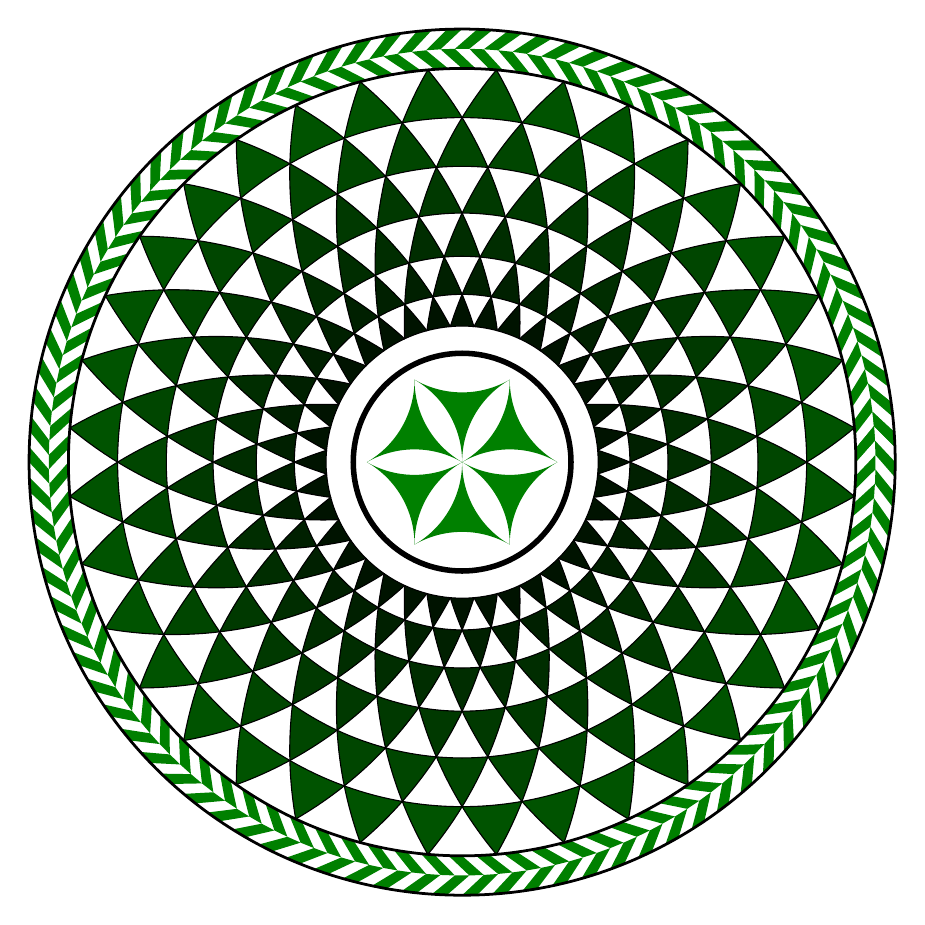
\begin{tikzpicture}[cap=round]
% Colors
\colorlet{anglecolor}{green!50!black}
\colorlet{bordercolor}{black}

%Configuration: change this to define number of intersections: 
% 5 degree mean 360/10 = 36 elements
\def\alpha{5} % degree
\def\layer{5}

\begin{scope}[scale=5]
% Radius R = 1

% The figure is constructed by intersecting circles Cx of radius R.
%  M_Cx lies on the circle C with a radius \alpha degree from the outer circle R 
%  and a distance defined by \alpha degree.

% It is sufficent to calculate one special M_C, which is intersecting the x-axis 
% at distance R from (0,0).
\pgfmathsetmacro\sinTriDiff{sin(60-\alpha)}
\pgfmathsetmacro\cosTriDiff{1-cos(60-\alpha)}
% The distance from the (0,0).
\pgfmathsetmacro\radiusC{sqrt(\cosTriDiff*\cosTriDiff + \sinTriDiff*\sinTriDiff)}
% Angle of M_C (from x-axis)
\pgfmathsetmacro\startAng{\alpha + atan(\sinTriDiff/\cosTriDiff)}

% The segment layer are \alpha degree apart
\pgfmathsetmacro\al{\alpha*\layer}

% For each segment create the intersection parts of the circles by using arcs
\foreach \x in {0,\alpha,...,\al}
{
  % Calculate the polar coordiantes of M_Cx. We take the M_C from above 
  % and  can calculate all other M_Cx by adding \alpha
  \pgfmathsetmacro\ang{\x + \startAng}
  % From ths we get the (x,y) coordinates
  \pgfmathsetmacro\xRs{\radiusC*cos(\ang)}
  \pgfmathsetmacro\yRs{\radiusC*sin(\ang)}

  % Now we intersect each new M_C with the x-axis:
  % We can find the radius of concentric inner circles
  \pgfmathsetmacro\radiusLayer{\xRs + sqrt( 1 - \yRs*\yRs )}

  % To calculate angles for the arcs later, this angle is needed
  \pgfmathsetmacro\angRs{acos(\yRs)}

 % We need to have the angle from the previous loop as well
  \pgfmathsetmacro\angRss{acos(\radiusC*sin(\ang-\alpha))}


  % Add some fading by \ang
  \colorlet{anglecolor}{black!\ang!green}

  % The loop needs to run a whole.  
  % We don't want to cope with angles > 360 degree, adapt the limits. 
  \pgfmathsetmacro\step{2*\alpha - 180}
  \pgfmathsetmacro\stop{180-2*\alpha}
  \foreach \y in {-180, \step ,..., \stop}
  {
    \pgfmathsetmacro\deltaAng{\y-\x}
    % This are the arcs which are definied by the intersection of 3 circles 
    \filldraw[color=anglecolor,draw=bordercolor] 
        (\y-\x:\radiusLayer)    
                arc (-90+\angRs+\deltaAng : \alpha-90+\angRss+\deltaAng :1) 
                arc (\alpha+90-\angRss+\deltaAng : 2*\alpha+90-\angRs+\deltaAng :1)
                arc (\deltaAng+2*\alpha : \deltaAng : \radiusLayer);
  }


  % helper circles  & lines
  %\draw[color=gray] (\xRs,\yRs) circle (1);
  %\draw[color=gray] (\xRs,-\yRs) circle (1);
  %\draw[color=blue] (0,0) circle (\radiusLayer);
  %\draw[color=blue, very thick] (0,0) -- (0:1);
  %\draw[color=blue, very thick] (0,0) -- (\ang:\radiusC) -- (\xRs,0);  
  %\draw[color=blue, very thick] (\xRs,\yRs) -- (0:\radiusLayer);
  %\filldraw[color=blue!20, very thick] (\xRs,\yRs) -- 
  % (\xRs,\yRs-0.3) arc (-90:-90+\angRs:0.2) -- cycle;

}
% Additional inner decoration element
\pgfmathsetmacro\xRs{\radiusC*cos(\al+\startAng)}
\pgfmathsetmacro\yRs{\radiusC*sin(\al+\startAng)}
\pgfmathsetmacro\radiusLayer{\xRs + sqrt( 1 - \yRs*\yRs )}
\draw[line width=2, color=bordercolor] (0,0) circle (.8*\radiusLayer);
\pgfmathsetmacro\radiusSmall{.7*\radiusLayer}
% There are six elements to create. Avoid angles >360 degree.
\foreach \x in {-60,0,...,240}
{
    \fill[color=anglecolor] (\x:\radiusSmall) arc (-180+\x+60: -180+\x: \radiusSmall)
                             arc (0+\x: -60+\x: \radiusSmall)
                             arc (120+\x: 60+\x: \radiusSmall); 
}
% The outer decoration
\foreach \x in {0, 4, ..., 360}
{
  \fill[color=anglecolor] (\x:1) -- (\x+3:1.05) -- (\x+5:1.05) -- (\x+2:1) -- cycle;
  \fill[color=anglecolor] (\x+5:1.05) -- (\x+7:1.05) -- (\x+4:1.1) -- (\x+2:1.1) -- cycle;
}
\draw[line width=1, color=bordercolor] (0,0) circle (1);
\draw[line width=1, color=bordercolor] (0,0) circle (1.1);
\end{scope}

\end{tikzpicture}

\end{document}
